\documentclass{beamer}
\usetheme[color=ACMblue]{ACMNew}
\usepackage{beamernotes}
\usepackage{algpseudocodex}
\usepackage{lipsum}
\usepackage{minted}
\usepackage{array}
\usepackage{tikz}
\usepackage{amsmath}
\usepackage{mathtools}
\usepackage{xcolor}
\usemintedstyle{manni}
\pdfcompresslevel=9
\pdfobjcompresslevel=3

\title[ACM fun]{CS 374B Review MT2}
\subtitle{Electric Boogaloo}
\author{ACM @ UIUC}
% \institute{The Mental Institute}  
\date{November 3, 2024}

\begin{document}

\begin{frame}
  \titlepage
\end{frame}
\bnote{This generates notes for pdfpc. These notes also appear
  on the handout/article versions.}

\begin{frame}[t]{Disclaimers and Logistics}
  \begin{itemize}
  \item \alert{Disclaimer:} Some of us are CAs, but we have not seen the exam. We have no idea what the questions are. However, we've taken the course and reviewed Kani's previous exams, so we have \alert{suspicions} as to what the questions will be like.
  \item This review session is being recorded. Recordings and slides will be distributed on EdStem after the end.
  \item \alert{Agenda:} We'll quickly review all topics likely to be covered, then go through a practice exam, then review individual topics by request.
  \begin{itemize}
      \item Questions are designed to be written in the same style as Kani's previous exams but to be \textit{slightly} harder, so don't worry if you don't get everything right away!
  \end{itemize}
  \item Please let us know if we're going too fast/slow, not speaking loud enough/speaking too loud, etc.
  \item If you have a question anytime during the review session, please ask! Someone else almost surely has a similar question.
  \item We'll provide a feedback form at the end of the session.
  \end{itemize}
\end{frame}

\begin{frame}[t]{Recursion}
  \begin{itemize}
    \item \alert{Definition:} Reducing the problem to a smaller instance of itself, where eventually we can terminate in a base case.
    \begin{itemize}
        \item Think: If we have a problem of size $n$, we want to continuously reduce to a problem smaller than $n$.
        \item Example: Tower of Hanoi
    \end{itemize}
    \begin{exampleblock}{Template}
        \begin{algorithmic}[1]
                \Procedure{AmazingRecursiveAlgo}{n}
                    \If {$n$ == [some base case]}
                        \State return [value]
                    \Else 
                        \State return \texttt{AmazingRecursiveAlgo}($n-1$)
                    \EndIf
                \EndProcedure
        \end{algorithmic}
        
    \end{exampleblock}
    \item Similar to \alert{induction}!
  \end{itemize}
\end{frame}

\begin{frame}[t]{Recursion: Runtime Analysis}
  \begin{itemize}
    \item \alert{General Form:} $$T(n) = \underbrace{r}_{\mathclap{\text{\# of subproblems}}} \; \cdot \; 
\overbrace{T\left(\frac{n}{c}\right)}^{\mathclap{\text{work at each subproblem}}} 
\; + \; \underbrace{f(n)}_{\mathclap{\text{work at current level}}}$$
    \begin{itemize}
        \item Describes how the amount of work changes between each level of recursion.
        \item We can solve for a \alert{time complexity} that describes the scaling behaviour of the algorithm at hand.
    \end{itemize}

    \pause
    \item \alert{Master's Theorem}
    \begin{block}{Master's Theorem}
        \begin{align*}
            \text{Decreasing: } r \cdot f(n / c) = \kappa \cdot f(n) \text{ where } \kappa < 1 &\implies T(n) = O(f(n)) \\ 
            \text{Equal: } r \cdot f(n / c) = \kappa \cdot f(n) \text{ where } \kappa = 1 &\implies T(n) = O(f(n)\cdot log_{c}{n}) \\
            \text{Increasing: } r \cdot f(n / c) = \kappa \cdot f(n) \text{ where } \kappa > 1 &\implies T(n) = O(n^{\log_{c}{r}})
        \end{align*}
    \end{block}
    \pause
    \begin{itemize}
        \item \alert{Intuition:} If each level contains more work than the level below it, then the root level will dominate. If each level contains the same amount of work, then we have $log_{c}{n}$ levels with $f(n)$ work. If each level contains less work than the work below it, then the leaf nodes will dominate.
    \end{itemize}
  \end{itemize}
\end{frame}

% Mergesort
\begin{frame}[t]{Divide and Conquer Algos: Merge Sort}
    \begin{itemize}
        \item \alert{Purpose:} Sort an arbitrary array.
        \item \alert{Time Complexity}: $O(n \log n)$
        \item \alert{Intuition:} Three phases: (a) split the array in half, (b) sort each side, (c) merge the sorted halves by repeatedly comparing smallest elements on each side not yet inserted.
        \begin{figure}
            \centering
            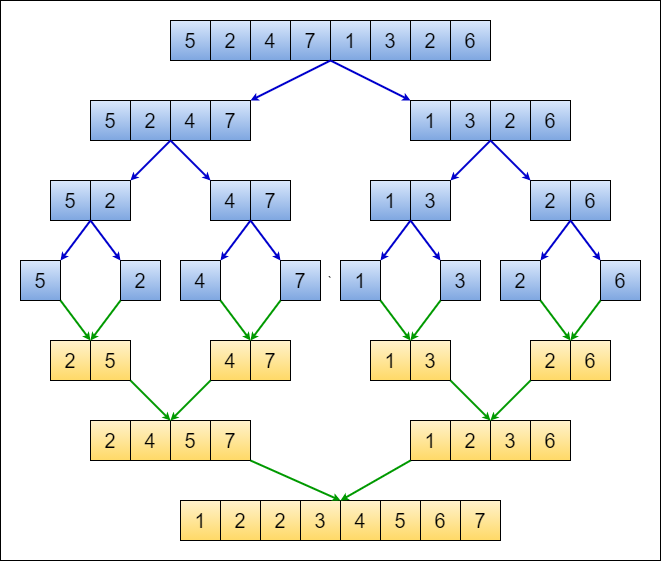
\includegraphics[width=0.5\linewidth]{mergesort.png}
        \end{figure}
    \end{itemize}
\end{frame}

% Quicksort
\begin{frame}[t]{Divide and Conquer Algos: Quicksort}
    \begin{itemize}
        \item \alert{Purpose:} Sort an arbitrary array.
        \item \alert{Time Complexity}: Avg: $O(n \log n)$ | Worst: $O(n^2)$ ($O(n \log n)$ deterministic with quickselect partitioning)
        \item \alert{Intuition}: Pick a pivot and rearrange the array such that all the elements that are less than the pivot value are to the left of the pivot value and all the elements that are greater than the pivot value are to the right of the pivot value. Then sort each side.   
        \begin{itemize}
            \item \alert{Why the poor worst case performance?}
            \item Because we can get unlucky and pick the worst possible pivot at every step.
        \end{itemize}
        \begin{figure}
            \centering
            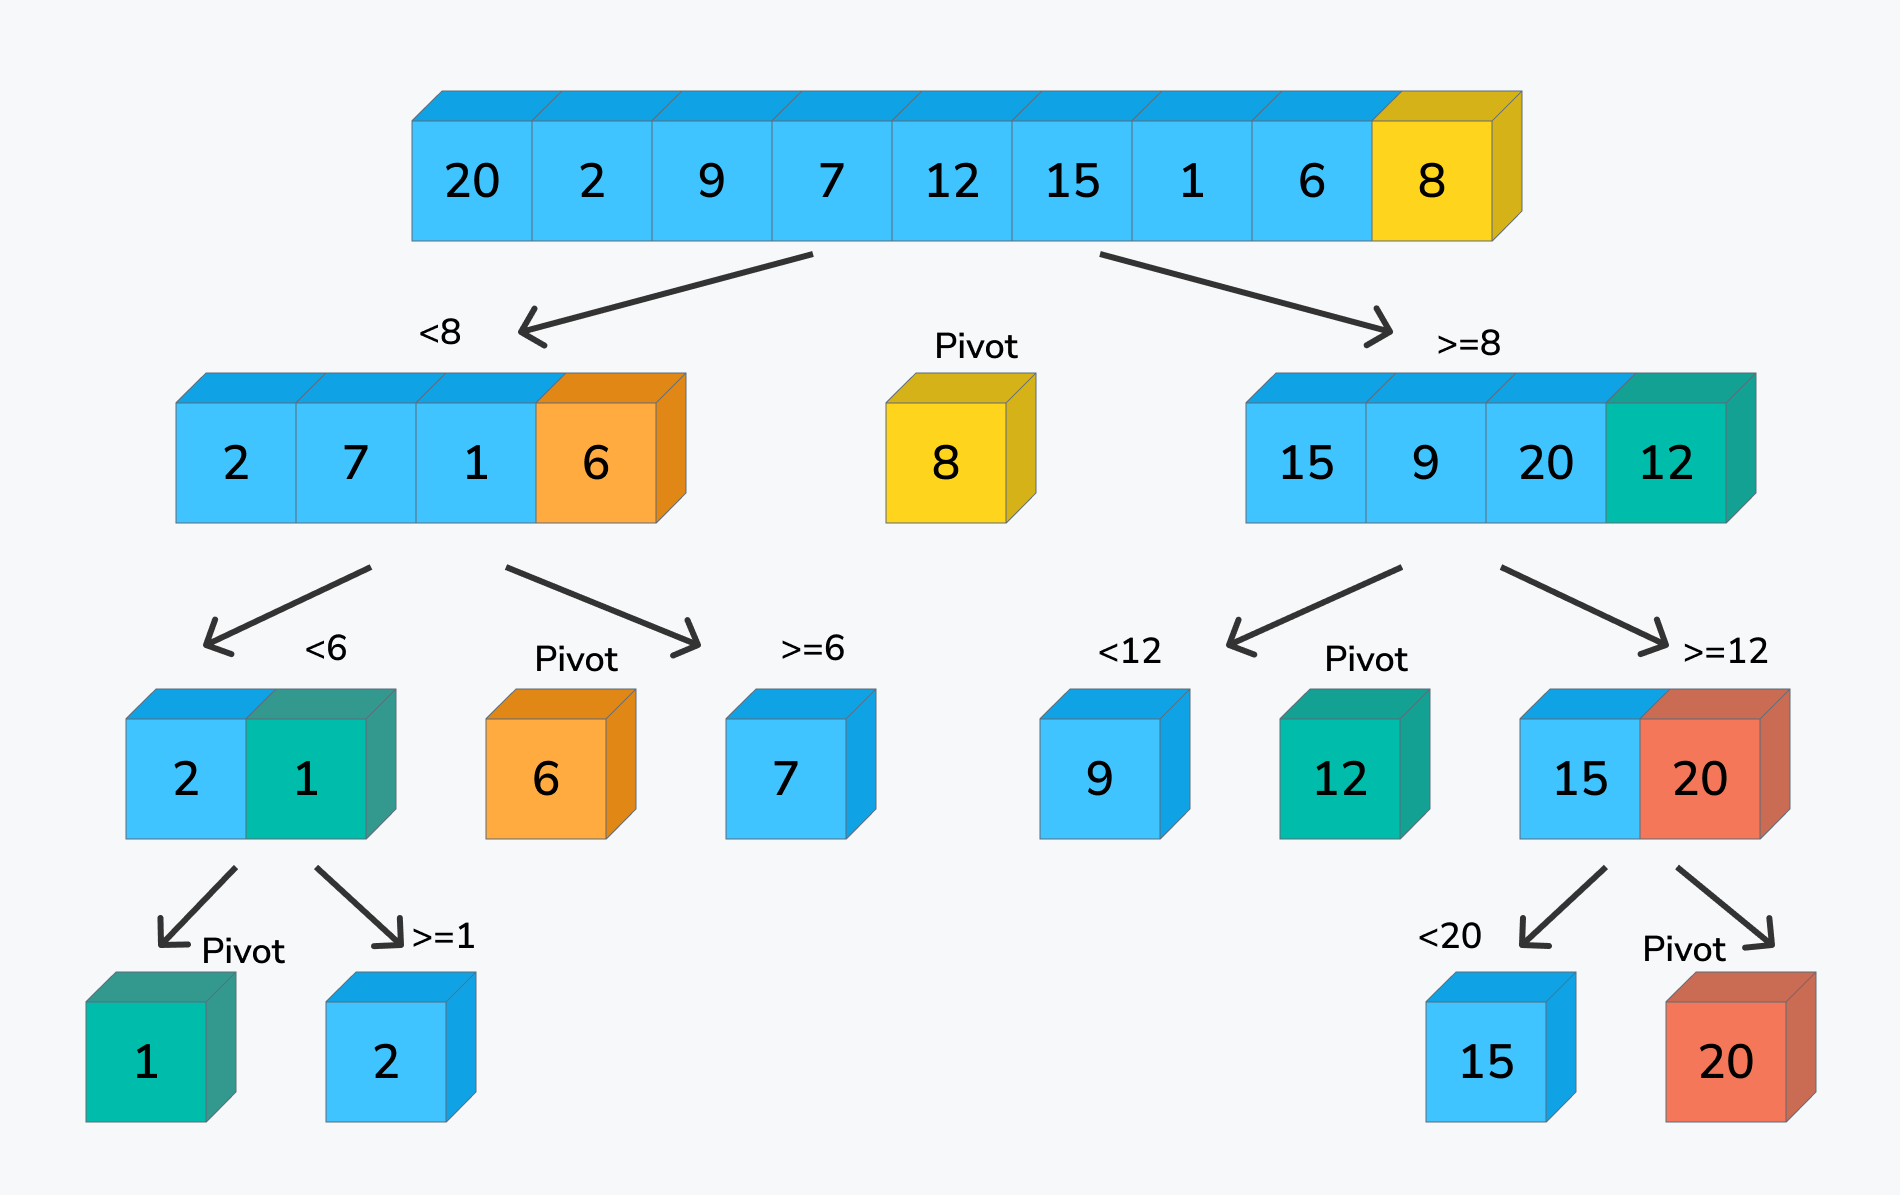
\includegraphics[width=0.5\linewidth]{quicksort.png}
        \end{figure}
    \end{itemize}
    \end{frame}

% Quickselect
\begin{frame}[t]{Divide and Conquer Algos: Quickselect}
    \begin{itemize}
        \item \alert{Purpose:} Get the $n^\text{th}$ smallest element in an arbitrary array.
        \item \alert{Time Complexity}: Avg: $O(n)$ | Worst; $O(n^2)$, ($O(n)$ with MoM)
        \item \alert{Intuition}: Pick a pivot $P$ with a value $P_V$ and rearrange the array such that all the elements that are less than $P_V$ are to the left of $P$ and all the elements that are greater than $P_V$ are to the right of P, just like quick select. If the length of the array of elements that are less than $P_V$ is greater than $n$, then we know that the $n^\text{th}$ smallest element is to the left of $P$ and we recurse on the left subarray. Otherwise, we know that the $n^\text{th}$ smallest element is to the right of $P$ and we recurse on the right subarray.
        \begin{itemize}
            \item \alert{Why the poor worst case performance?}
            \item Again, because we can get unlucky and pick the worst possible pivot at every step.
            \item We can guarantee linear performance with a better pivot-picking algorithm such as \textsc{MedianOfMedians}
            \begin{itemize}
                \item Finds element that larger than $\frac{3}{10}$ and smaller than $\frac{7}{10}$ of the array's elements.
                \item Runs in $O(n)$ time
            \end{itemize}
        \end{itemize}
    \end{itemize}
\end{frame}

% Binary Search
\begin{frame}[t]{Divide and Conquer Algos: Binary Search}
    \begin{itemize}
        \item \alert{Purpose:} Find the existence of an element in a sorted array
        \item \alert{Time Complexity}: $O(\log n)$
        \item \alert{Intuition}: Say we are trying to find the value $n$. Pick the middle element $M$ in the array. If $n > M$, the element must be to the right of $n$ and we recurse on the right. Otherwise, we recurse on the left.
    \end{itemize}
    \begin{figure}
        \centering
        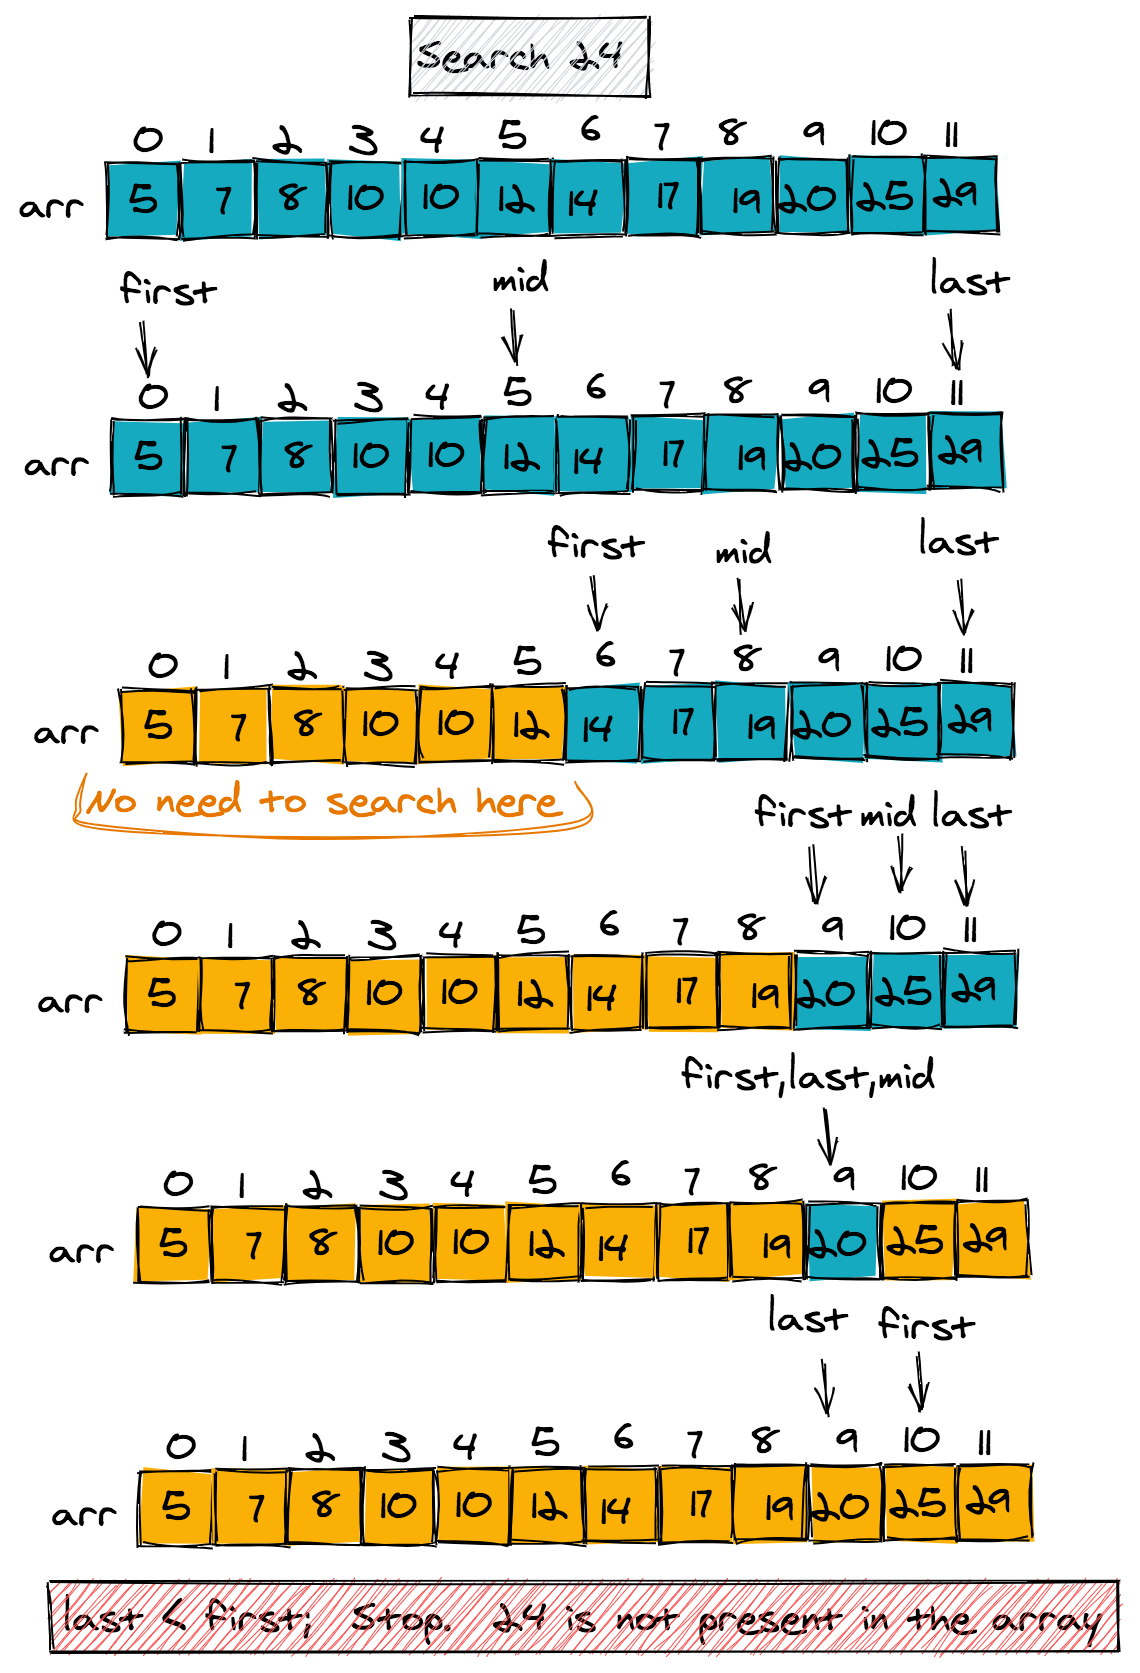
\includegraphics[width=0.25\linewidth]{binary.png}
    \end{figure}
\end{frame}


% Karatsubas
\begin{frame}[t]{Divide and Conquer Algos: Karatsuba's}
    \begin{itemize}
        \item \alert{Purpose:} Multiplication
        \item \alert{Time Complexity}: $O(n^{\log_2{3}}) \approx O(n^{1.585})$
        \item 3 Phases:
        \begin{itemize}
            \item \alert{Divide}: Represent $x$ as $x_0 p^n + x_1$, $y$ as $y_0 p^n + y_1$
            \item \alert{Recurse}: Calculate $x_0y_0$, $x_1y_1$, $(x_0 + x_1)(y_0 + y_1)$
            \item \alert{Combine}: Use the three results to calculate our final answer.
        \end{itemize}
        
    \end{itemize}
    \begin{figure}
        \centering
        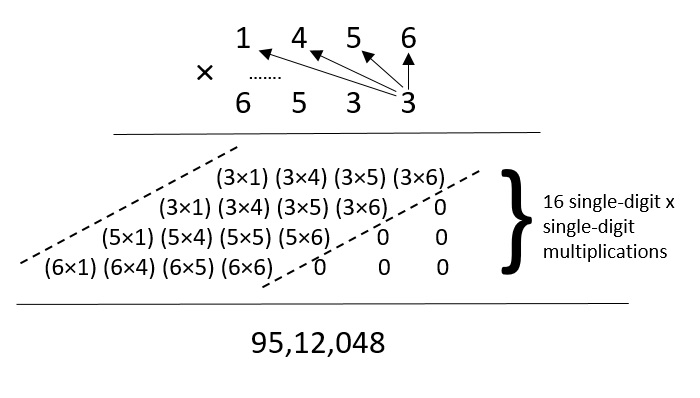
\includegraphics[width=0.5\linewidth]{karatsuba.png}
    \end{figure}
\end{frame}


\begin{frame}[t]{Backtracking}
    \begin{itemize}
        \item Technique to methodically explore the solutions to a problem via the reduction to said problem to a \underline{smaller} variant of itself, a.k.a \alert{recursion}. 
        % This intuition might just be a me thing lmao
        \item Intuitively, think of the problem space as a maze that we are trying to find the exit of. For each path, you would traverse until you reach a dead end, at which point you \alert{back track} to try a different path.
        \item To find recurrence, think ''What information about a subset of my current problem space would be really nice to know?''
    \pause
    \alert{Example:} Longest Increasing Subsequence
        \item ''What is the length of a longest increasing subsequence in an arbitrary array?''
    \end{itemize}
    \pause
    \begin{align*}
        \text{LIS}(i, j) = \begin{cases}
        0 & \text{if } i = 0 \\
        \text{LIS}(i - 1, j) & \text{if } A[i] \geq A[j] \\
        \max \begin{cases}
            \text{LIS}(i -1, j) \\
            1 + \text{LIS}(i - 1, i)
        \end{cases} & \text{else}
    \end{cases}
    \end{align*}
    \pause
    This kind of sucks; we're redoing computation that we've already done! What if instead, we computed all the subproblems beforehand, wrote down the solutions, then did the recursion?
\end{frame}

\begin{frame}[t]{Dynamic Programming}
  \begin{itemize}
      \item It's backtracking, but we compute all of the subproblems iteratively.
      \begin{itemize}
          \item This idea of "writing things down" as to not repeat computation is called \alert{memoization} 
      \end{itemize}   
      \pause
      \item Alternatively, you can think about this recursively, except we check our memoization structure to see if we've computed anything before. If we have, we just use the computed result. Otherwise, we compute the subproblem.
      \pause
      \item For a DP solution, we need:
      \begin{enumerate}
            \item English Description
            \item Recurrence
            \item Memoization Structure
            \item Solution Location
            \item Evaluation Order
            \item Runtime
      \end{enumerate}
      \pause
      \item \alert{How to solve a DP:}
      \begin{itemize}
          \item Identify how we can take advantage of a recursive call on a smaller subset of the input space.
          \item Identity base cases
          \item Identity recurrences (they should cover all possible cases at each step)
      \end{itemize}
  \end{itemize}
\end{frame}

\begin{frame}[t]{Dynamic Programming}
  Let's look at the LIS example from before:
  ''What is the length of a longest increasing subsequence in an arbitrary array?''
  \pause
  \begin{figure}
      \centering
      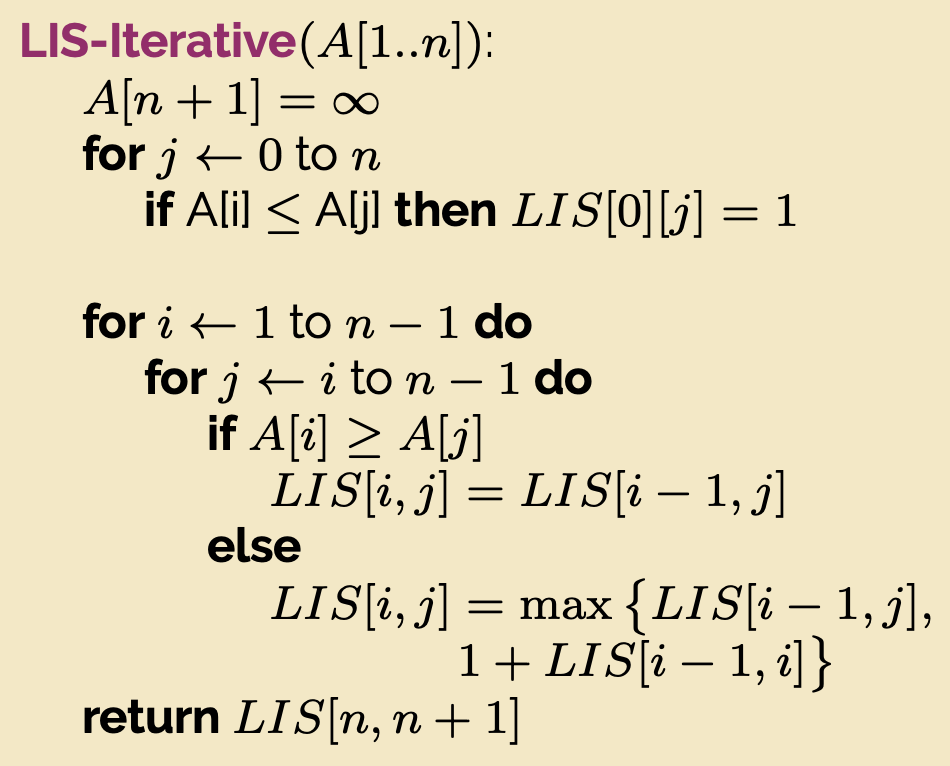
\includegraphics[width=0.5\linewidth]{dp.png}
  \end{figure}
\end{frame}

\begin{frame}[t]{Graphs}
  \begin{itemize}
      \item \alert{Definition:} A set of vertices $V$ connected by a set of edges $E$. Individual edges are notated as $(u, v)$, where $u, v \in V$.
      \begin{itemize}
          \item They are usually represented as \alert{adjacency lists} or \alert{adjacency matrices} \pause
          \item \alert{Directed:} Each edge $(u, v) \in E$ now has a direction $u \to v$ \pause
          \item \alert{Acyclic:} No cycles. \pause
      \end{itemize}
      \item \alert{Path:} A sequence of distinct vertices where each pair of consecutive vertices have an edge \pause
      \item \alert{Cycle:} A sequence of distinct vertices where each pair of consecutive vertices have an edge \textbf{and} the first and last vertices are connected. \pause
      \item \alert{Connected:} $u, v \in V$ are connected $\iff$ there exists a path between $u$ and $v$. \pause
      \item \alert{Strongly Connected:} $u, v \in V$ are strongly connected $\iff$ there exists a path between $u$ and $v$ and from $v$ to $u$. \pause
      
      \item \alert{Connected Component (of $u$):} The set of all vertices connected to $u$. \pause
      \item \alert{Strongly Connected Component:} A set of vertices a strongly connected component if each pair of vertices are strongly connected. \pause
      
  \end{itemize}
\end{frame}

\begin{frame}[t]{Graph Algorithms: Traversal}
  \begin{itemize}
    \pause
      \item \alert{BFS:} 
      \begin{itemize}
          \item \alert{Purpose:} Reachability, Shortest Path (unweighted graph)
          \item \alert{Implementation details:} Add your neighbours to a \alert{queue}, pop from the queue to get next node
          \item \alert{Runtime:} $O(V + E)$
      \end{itemize}
    \pause
      \item \alert{DFS:} 
      \begin{itemize}
          \item \alert{Purpose:} Reachability, toposort 
          \item \alert{Implementation details:} Add your neighbours to a \alert{stack}, pop from the stack to get next node
          \item \alert{Runtime:} $O(V + E)$
      \end{itemize}
  \end{itemize}
\end{frame}

\begin{frame}[t]{Graph Algorithms: Shortest Path}
  \begin{itemize}
  \pause
    \item \alert{Dijkstra's}
    \begin{itemize}
        \item \alert{Purpose:} SSSP, no negative edges
        \item \alert{Implementation:} Visit neighbours in \alert{priority queue}
        \item \alert{Runtime:} $O(m+n \log n)$
    \end{itemize}
    \pause
    \item \alert{Bellman-Ford:}
    \begin{itemize}
        \item \alert{Purpose:} SSSP, yes negative weights. Will detect negative cycles.
        \item \alert{Implementation:} Dynamic Programming recurrence
        \item \alert{Runtime:} $O(mn)$
    \end{itemize}
    \pause
    \item \alert{Floyd-Warshall:}
    \begin{itemize}
        \item \alert{Purpose:} APSP, yes negative edge weights
        \item \alert{Implementation:} Dynamic Programming recurrence
        \item \alert{Runtime:} $O(n^3)$
    \end{itemize}
  \end{itemize}
\end{frame}

 \begin{frame}[t]{Graph Algorithms: MSTs}
   3 main algorithms:
   \begin{itemize}
       \item \alert{Prim-Jarnik}: Keep a priority queue for edges to be added to the tree. Start the tree at some arbitrarily selected root vertex. When adding a vertex, add all of its neighbors to the queue. Runtime: $O(|E| \log |V|)$, $O(|V| \log |V| + |E|)$ using Quake heaps.
       \item \pause \alert{Kruskal}: Keep a disjoint-sets data structure to keep track of connected components. Sort the edges, then in order, add each edge if it connects two components. Runtime: $O(|E| \log |V|)$.
       \item \pause \alert{Bor\r{u}vka}: No fancy data structures! Just find smallest edge going out of each vertex, then contract all edges that you selected! Runtime: $O(|E| \log |V|)$
       \item \pause Faster (but way more complicated algorithms) exist. \alert{Yao} (1975): $O(|E| \log \log |V|)$ with a modification of Bor\r{u}vka's (using linear-time median selection). \alert{Karger-Klein-Tarjan} (1995): $O(|E|)$ in expectation, \alert{Chazelle} (2000): $O(|E| \alpha(|V|, |E|))$ deterministic
   \end{itemize}
 \end{frame}

\begin{frame}[t]{Graph Algorithms: SCC}
  \alert{SCC-Finding Algorithms (Tarjan's, Kosuraju's)}
  \begin{itemize}
      \item \alert{Purpose:} To identify (and collapse) SCCs in a (directed) graph
      \item \alert{Runtime:} $O(V + E)$
      \item \alert{Returns:} A metagraph that has one node for each SCC.
  \end{itemize}
  \begin{figure}
      \centering
      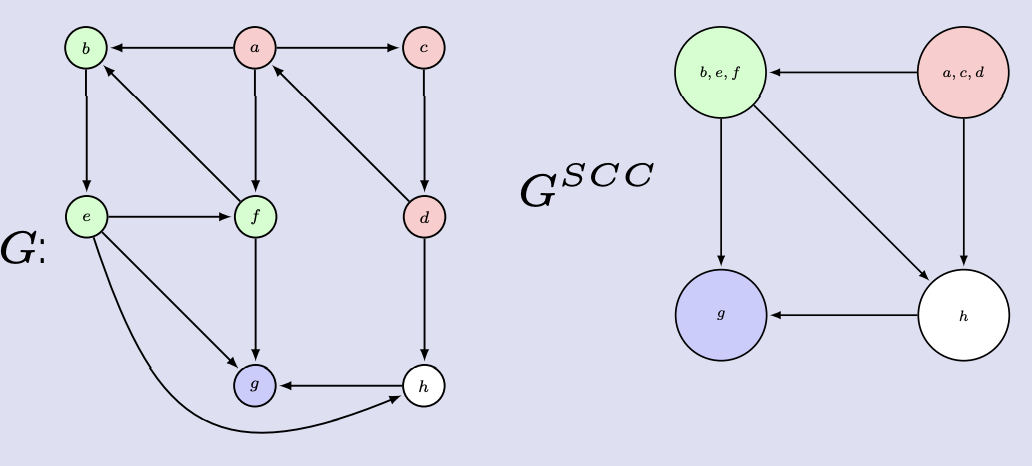
\includegraphics[width=0.5\linewidth]{SCC.png}
  \end{figure}
\end{frame}

\begin{frame}[t]{Graph Problems: General Stuff}
  \alert{How to solve graph problems:}
  \begin{enumerate}
        \item Identify type of problem (Reachability, Shortest Path, SCC)
        \item Construct new graph
        \begin{itemize}
            \item Add sources/sinks
            \item Add vertices via $V' = V \times \{\text{some set}\}$ (Useful for tracking states)
            \item Add vertices via $E' = E \times \{\text{some set}\}$ (Useful for allowing/prohibit certain behaviour)
        \end{itemize}
        \item Apply some stock algorithm
        \item Draw connection between how to result of the algorithm upon the new graph relates to the solution of the original question.
  \end{enumerate}
\end{frame}

\begin{frame}[t]{Recurrences and Asymptotics}
    Give a tight asymptotic bound for each recurrence:
    \begin{itemize}
        \item $T(n) = 4\>T(\frac{n}{2}) + n \log_2 n$
        \item \pause $T(n) = T(\frac{3n}{4}) + T(\frac{n}{4}) + 5n$
        \item \pause $T(n) = 9\> T(\frac{n}{3}) + n^2$
    \end{itemize}    
    \pause Group the following functions s.t. $f$ and $g$ are in the same group if $f(x) \sim \Theta(g(x))$, and sort the groups by runtime:
    \begin{itemize}
        \item $n^n$
        \item $\log \log n$ 
        \item $374^n$
        \item $n!$
        \item $\log (n + n^{374})$ 
        \item $\log n^n$
        \item $n^{1.000001}$
        \item $2^n$
        \item $n \log n^5$
        \item $\frac{1}{\log_n 2}$
    \end{itemize}
    
\end{frame}

\begin{frame}[t]{Divide and Conquer}

Consider the following (correct!) in-place sorting algorithm:

\begin{algorithmic}[1]
    \Procedure{StoogeSort}{$A[1\dots n]$}
        \State If $A[1] > A[n]$, swap them.
        \If {$n \ge 3$}
            \State \Call{StoogeSort}{} the initial $2/3$ of $A$
            \State \Call{StoogeSort}{} the final $2/3$ of $A$
            \State \Call{StoogeSort}{} the initial $2/3$ of $A$ (again)
        \EndIf
    \EndProcedure
\end{algorithmic}

Give a \emph{tight} asymptotic bound on the runtime of StoogeSort, in terms of $n$.

\end{frame}

\begin{frame}[t]{Graphs}

Given a program represented as a directed graph $G = (V, E)$ and function $R$ where:
\begin{enumerate}[-]
    \item Each vertex $v \in V$ represents a function
    \item Each edge $u \to v \in E$ represents that function $u$ can call $v$ internally
    \item $R(v)$ represents the "resource" that function $v$ has \emph{exclusive} access to during execution. $R(v) \in \{1, 2, \dots k\}$.
\end{enumerate}

You are given the "\texttt{main} function" $s \in V$. Considering that an execution path cannot have two functions using the same resource at the same time, write an algorithm to find the set $D \subseteq V$ of functions that could not possibly be called as a result of running $s$.


\end{frame}

\begin{frame}[t]{Dynamic Programming}

You are given an array of integers $A[1..2n]$. On each turn, you choose two arbitrary integers with no other numbered integers between them. You then earn points equal to the division of your two chosen numbers, and both chosen integers are removed. Once a square is removed, it cannot be chosen in any future turns. Your goal is to remove all of the numbers and to earn as many points as possible. Describe an algorithm to find the maximum number of points you can earn in a game. 
\renewcommand{\arraystretch}{1.5} % Adjust row height

\begin{center}
\begin{tabular}{|>{\centering\arraybackslash}p{0.5cm}
                |>{\centering\arraybackslash}p{0.5cm}
                |>{\centering\arraybackslash}p{0.5cm}
                |>{\centering\arraybackslash}p{0.5cm}
                |>{\centering\arraybackslash}p{0.5cm}
                |>{\centering\arraybackslash}p{0.5cm}
                |>{\centering\arraybackslash}p{0.5cm}
                |>{\centering\arraybackslash}p{0.5cm}
                |>{\centering\arraybackslash}p{0.5cm}
                |>{\centering\arraybackslash}p{0.5cm}
                |>{\centering\arraybackslash}p{0.5cm}
                |>{\centering\arraybackslash}p{0.5cm}
                |}
    \hline
    4 & 3 & 6 & 5 & 9 & 1 & 2 & 3 & \textcolor{red}{7} & \textcolor{red}{3} & 4 & 8 \\
    \hline
    4 & 3 & 6 & 5 & \textcolor{red}{9} & \textcolor{red}{1} & 2 & 3 &  &  & 4 & 8 \\
    \hline
    4 & 3 & 6 & \textcolor{red}{5} &  &  &\textcolor{red}{2} & 3 &  &  & 4 & 8 \\
    \hline
    4 & 3 & \textcolor{red}{6} &  &  &  &  & \textcolor{red}{3} &  &  & 4 & 8 \\
    \hline
    \textcolor{red}{4} & \textcolor{red}{3} &  &  &  &  &  &  &  &  & 4 & 8 \\
    \hline
      &  &  &  &  &  &  &  &  &  & \textcolor{red}{4} & \textcolor{red}{8} \\
    \hline
    \end{tabular}
\hspace{1cm}
\begin{tabular}{l}\\
    + $\frac{7}{3}$ points! \\
    + $\frac{9}{1}$ points! \\
    + $\frac{5}{2}$ points! \\
    + $\frac{6}{3}$ points! \\
    + $\frac{4}{3}$ points! \\
    + $\frac{4}{8}$ points! \\
    All done!
\end{tabular}
\end{center}

\end{frame}

\begin{frame}[t]{Graphs}
    %Easier variant for B-section
    It's late at night, and you're walking home. You have a (directed, weighted) graph $G = (V, E)$ describing Champaign's road network, with each edge annotated as to whether or not the edge is lit by streetlights. Describe and analyze an efficient algorithm to calculate the shortest $s \rightarrow t$ path for a given $(s, t)$, where at most $k$ edges are unlit.
\end{frame}

%\begin{frame}[t]{Graphs}
%    You are in Austin, TX, which is lit at night by ``moon towers'', high powerful lamps which illuminate multiple blocks. You are given a weighted undirected graph $G = (V,E)$ as a map of Austin, as well as a list of moon towers represented as pairs $(p, v)$ where $v \in V$ is the location of the tower and $p \in \mathbb{R}_+$ is the \textit{power} of the moon tower, indicating that everywhere within distance $p$ of the tower will be lit. Describe and analyze an efficient algorithm to calculate the shortest $s \rightarrow t$ path for a given $(s, t)$, where all edges are entirely illuminated by moon towers.

%    \begin{figure}
%        \centering
%        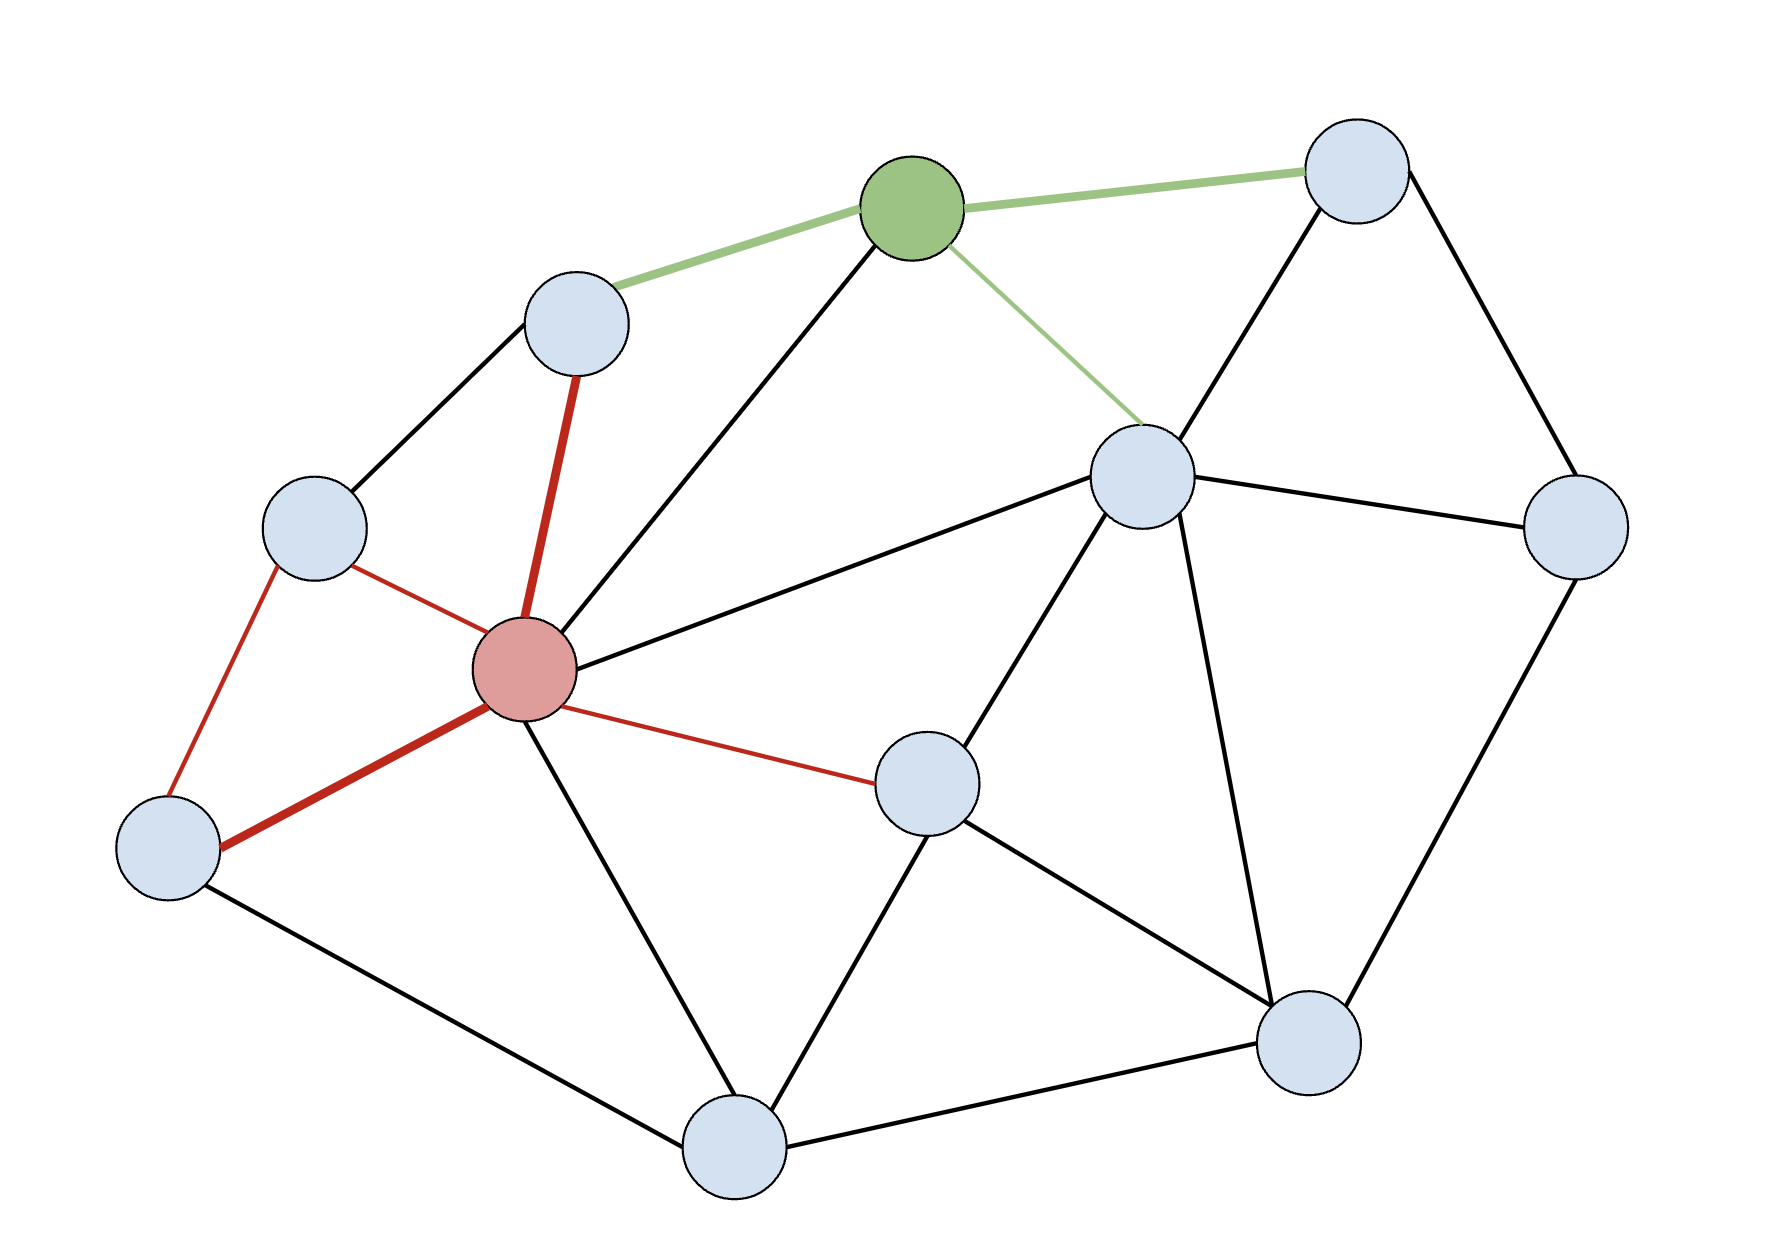
\includegraphics[width=0.5\linewidth]{moontower_graph.png}
%    \end{figure}
%\end{frame}

\end{document}
